% debut d'un fichier latex standard
\documentclass[a4paper,12pt,twoside]{article}

\usepackage{lipsum}
\usepackage{empheq}

% pour l'inclusion de figures en eps,pdf,jpg
\usepackage{graphicx}
\usepackage{subcaption}
\usepackage{wrapfig}
% quelques symboles mathematiques en plus
\usepackage{amsmath}
\usepackage{amsthm} % Pour les preuves
\usepackage{cancel} % Pour barrer des trucs en mode math
% le tout en langue francaise
%\usepackage[french]{babel}
% on peut ecrire directement les caracteres avec l'accent
% a utiliser sur Linux/Windows
\usepackage[utf8]{inputenc}
\usepackage[T1]{fontenc}
% a utiliser sur le Mac
%\usepackage[applemac]{inputenc}
% pour l'inclusion de links dans le document
\usepackage[colorlinks,bookmarks=false,linkcolor=blue,urlcolor=blue]{hyperref}
\usepackage{siunitx}
% pour les degrés
\usepackage{textcomp}
\paperheight=297mm
\paperwidth=210mm

\setlength{\textheight}{235mm}
\setlength{\topmargin}{-1.2cm} % pour centrer la page verticalement
%\setlength{\footskip}{5mm}
\setlength{\textwidth}{15cm}
\setlength{\oddsidemargin}{0.56cm}
\setlength{\evensidemargin}{0.56cm}

\pagestyle{plain}

% quelques abreviations utiles
\def \be {\begin{equation}}
\def \ee {\end{equation}}
\def \dd  {{\rm d}}

\newcommand{\mail}[1]{{\href{mailto:#1}{#1}}}
\newcommand{\ftplink}[1]{{\href{ftp://#1}{#1}}}

\newcommand{\illabel}[1]{ ~ \refstepcounter{equation}(\theequation)\label{#1}} % Ecrit une équation dans le texte, numérotés.
\newcommand{\mbf}[1]{\mathbf{#1}} % bold font in math
\newcommand{\grad}[1]{\nabla#1}
\newcommand{\Div}[1]{\nabla\cdot\mathbf{#1}}
\newcommand{\rot}[1]{\nable\cross\mathbf{#1}}
\newcommand{\bracket}[1]{\left(#1\right)}
\newcommand{\sqbracket}[1]{\left[#1\right]}
\newcommand{\lapl}[1]{\Delta#1}

%
% latex SqueletteRapport.tex      % compile la source LaTeX
% xdvi SqueletteRapport.dvi &     % visualise le resultat
% dvips -t a4 -o SqueletteRapport.ps SqueletteRapport % produit un PostScript
% ps2pdf SqueletteRapport.ps      % convertit en pdf

% pdflatex SqueletteRapport.pdf    % compile et produit un pdf
% \message{================> TAILLE DE LA POLICE EN CM \printinunitsof{cm}\prntlen{\textwidth}}

% ======= Le document commence ici ======

\begin{document}
% Le titre, l'auteur et la date
\title{Wave equation in an inhomogeneous environment\\{\normalsize Normal modes and propagation of the wave of a tsunami}\\{\small Physique Numérique I}\\{\small Rapport 7}}
\date{\today}
\author{Delphine Martres and Damien Korber\\{\small \mail{delphine.martres@epfl.ch} and \mail{damien.korber@epfl.ch}}}

\maketitle
\tableofcontents % Table des matieres


% Quelques options pour les espacements entre lignes, l'identation
% des nouveaux paragraphes, et l'espacement entre paragraphes
\baselineskip=16pt
\parindent=15pt
\parskip=5pt
\newpage

%%%% ON COMMENCE A ECRIRE D'ICI

%===============================================================================
%=============================== INTRODUCTION ==================================
%===============================================================================
\section{Introduction}
  This report will focus on the study of the behaviour of waves in an unidimensional environment.
  These waves will be governed by equations \eqref{eq:ondes-ABC}.

  \begin{align}
    \begin{split}
      \text{Equation A: }&~\frac{\partial^2f}{\partial t^2}=u^2\frac{\partial^2f}{\partial x^2}\\
      \text{Equation B: }&~\frac{\partial^2f}{\partial t^2}=\frac{\partial}{\partial x}\bracket{u^2\frac{\partial f}{\partial x}}\\
      \text{Equation C: }&~\frac{\partial^2f}{\partial t^2}=\frac{\partial^2}{\partial x^2}\bracket{u^2f}
    \end{split}
    \label{eq:ondes-ABC}
  \end{align}

  The domain considered is $x\in\left[0,L\right]$ with different border condition depending on the situation.
  The initial condition is given by $f(x,t=0)=0~\forall x$.




%===============================================================================
%=========================== IMPLEMENTATION ====================================
%===============================================================================
\section{Implementation}
  \subsection{Discretization of the waves equations}

  To discretize equations \eqref{eq:ondes-ABC}, an explicit 3-levels numerical method will be used.
  This means that for any function $g(x)$ twice-differentiable, we get equation \eqref{eq:3-levels-method}.

  \begin{equation}
    \frac{\partial g}{\partial x}(x_i)\approx\frac{g(x_{i+1}) - g(x_{i-1})}{2h}~\text{ and }~\frac{\partial^2 g}{\partial x^2}(x_i)\approx\frac{g(x_{i+1}) - 2g(x_i) + g(x_{i-1})}{h^2}
    \label{eq:3-levels-method}
  \end{equation}

  with $h=x_{i+1} - x_i$.
  Thus, the resulting discretization of the waves equations gives equations \eqref{eq:onde-A-disc}, \eqref{eq:onde-B-disc} and \eqref{eq:onde-C-disc}.
  Note that $f_i^n \equiv f(x_i, t_n)$ and $u_i \equiv u(x_i)$.

  \begin{align}
    \intertext{Equation A:}
    \Aboxed{f^{n+1}_i &= 2f^n_i - f^{n-1}_i + \bracket{\frac{\Delta t}{\Delta x}}^2u^2_i\sqbracket{f^n_{i+1} - 2f^n_i + f^n_{i-1}}}\label{eq:onde-A-disc}
    \intertext{Equation B:}
    \Aboxed{f^{n+1}_i &= 2f^n_i - f^{n-1}_i + \bracket{\frac{\Delta t}{\Delta x}}^2u^2_i\sqbracket{f^n_{i+1} - 2f^n_i + f^n_{i-1}} + \bracket{\frac{\Delta t}{\Delta x}}^2\frac{u_i}{2}(u_{i+1}-u_{i-1})(f^n_{i+1}-f^n_{i-1})}\label{eq:onde-B-disc}
    \intertext{Equation C:}
    \Aboxed{f^{n+1}_i &= 2f^n_i - f^{n-1}_i + \bracket{\frac{\Delta t}{\Delta x}}^2\sqbracket{u^2_{i+1}f^n_{i+1} - 2u^2_if^n_i + u^2_{i-1}f^n_{i-1}}} \label{eq:onde-C-disc}
  \end{align}

  \subsection{Border conditions}
    Multiple border conditions are given for this exercice.
    Furthermore, both side must be separated.
    Note that $u(x) \geq 0~\forall x$ and $f_i^n \equiv f(x_i, t_n)$ and $u_i \equiv u(x_i)$.

    \subsubsection{Left border}
      \paragraph{Fixed.}
        The left fixed condition is simply given by $\boxed{f^{n+1}_0 = f^n_0}$.
      \paragraph{Free.}
      \lipsum[1] %TODO : Virer quand y'a le texte. C'est pour mettre de la structure.
      %TODO : À remplir
      \paragraph{Harmonic.}
      \lipsum[1] %TODO : Virer quand y'a le texte. C'est pour mettre de la structure.
      %TODO : À remplir
      \paragraph{Exit.}
        \begin{align}
          \intertext{For the left exit, $f$ is given by a strictly backward wave.}
          f(x,t) &= G(x+ut)~\forall x~\forall t
          \intertext{Thus:}
          \frac{\partial f}{\partial t}(x_L, t) &= uG' = u(x_L)\frac{\partial f}{\partial x}(x_L,t) \forall t
          \intertext{By using a forward finite difference for both $x$ and $t$:}
          \frac{f_0^{n+1} - f_0^{n}}{\Delta t} &= u_0\frac{f_1^n - f_0^n}{\Delta x}
          \intertext{Which leads to the left exit border condition.}
          \Aboxed{ f_0^{n+1} &= u_0\frac{\Delta t}{\Delta x}\sqbracket{f_1^n - f_0^n} + f_0^n}\label{eq:left-exit}
        \end{align}

    \subsubsection{Right border}
      \paragraph{Fixed.}
      The right fixed condition is simply given by $\boxed{f^{n+1}_{N} = f^n_N}$. %TODO : C'est juste ça ?
      \paragraph{Free.}
      \lipsum[1] %TODO : Virer quand y'a le texte. C'est pour mettre de la structure.
      %TODO : À remplir
      \paragraph{Harmonic.}
      \lipsum[1] %TODO : Virer quand y'a le texte. C'est pour mettre de la structure.
      %TODO : À remplir
      \paragraph{Exit.}
      \begin{align}
        \intertext{For the right exit, $f$ is given by a strictly forward wave.}
        f(x,t) &= F(x-ut)~\forall x~\forall t
        \intertext{Thus:}
        \frac{\partial f}{\partial t}(x_R, t) &= -uF' = -u(x_R)\frac{\partial f}{\partial x}(x_R,t) \forall t
        \intertext{By using a forward finite difference for $t$ and a backward finite difference for $x$:}
        \frac{f_N^{n+1} - f_N^{n}}{\Delta t} &= -u_N\frac{f_N^n - f_{N-1}^n}{\Delta x}
        \intertext{Which leads to the right exit border condition.}
        \Aboxed{ f_N^{n+1} &= -u_N\frac{\Delta t}{\Delta x}\sqbracket{f_N^n - f_{N-1}^n} + f_N^n}\label{eq:left-exit}
      \end{align}

    %TODO : À remplir


  \subsection{Energy of the wave}
    The energy of a wave over a domain $x\in\left[0, L\right]$ is given by equation \eqref{eq:energie-continue}.

    \begin{equation}
      E(t) = \int_0^L f^2(x,t)dx
      \label{eq:energie-continue}
    \end{equation}

    An estimation of the integral of any integrable function $g$ can be found using the trapezoidal rule, which is given by equation \eqref{eq:trapeze-rule}.

    \begin{equation}
      \int_a^b g(x)dx \approx h\sum_{i=1}^N\bracket{\frac{g(x_i) + g(x_{i+1})}{2}}
      \label{eq:trapeze-rule}
    \end{equation}

    with $h = x_{i+1} - x_i$.
    Thus, the energy is given by equation \eqref{eq:energie-discret}.

    \begin{equation}
      \boxed{E(t) = (\Delta x)\sum_{k=0}^{N-2}\frac{f^2(x_k) + f^2(x_{k+1})}{2}}\\
      \label{eq:energie-discret}
    \end{equation}

    \newpage

    \section{Constant propagation speed}
    In this section, $u(x)=const=6$ (which implies equations \eqref{eq:ondes-ABC} are equal) m/s and $L=20$ m.

    \subsection{Border reflection}
    The left border condition is $f(0,t)=A\sin(\omega t)$ with $A=1$ m and $\omega=5$ rad/s.

    \begin{figure}[h!]
    \begin{subfigure}{0.5\textwidth}
    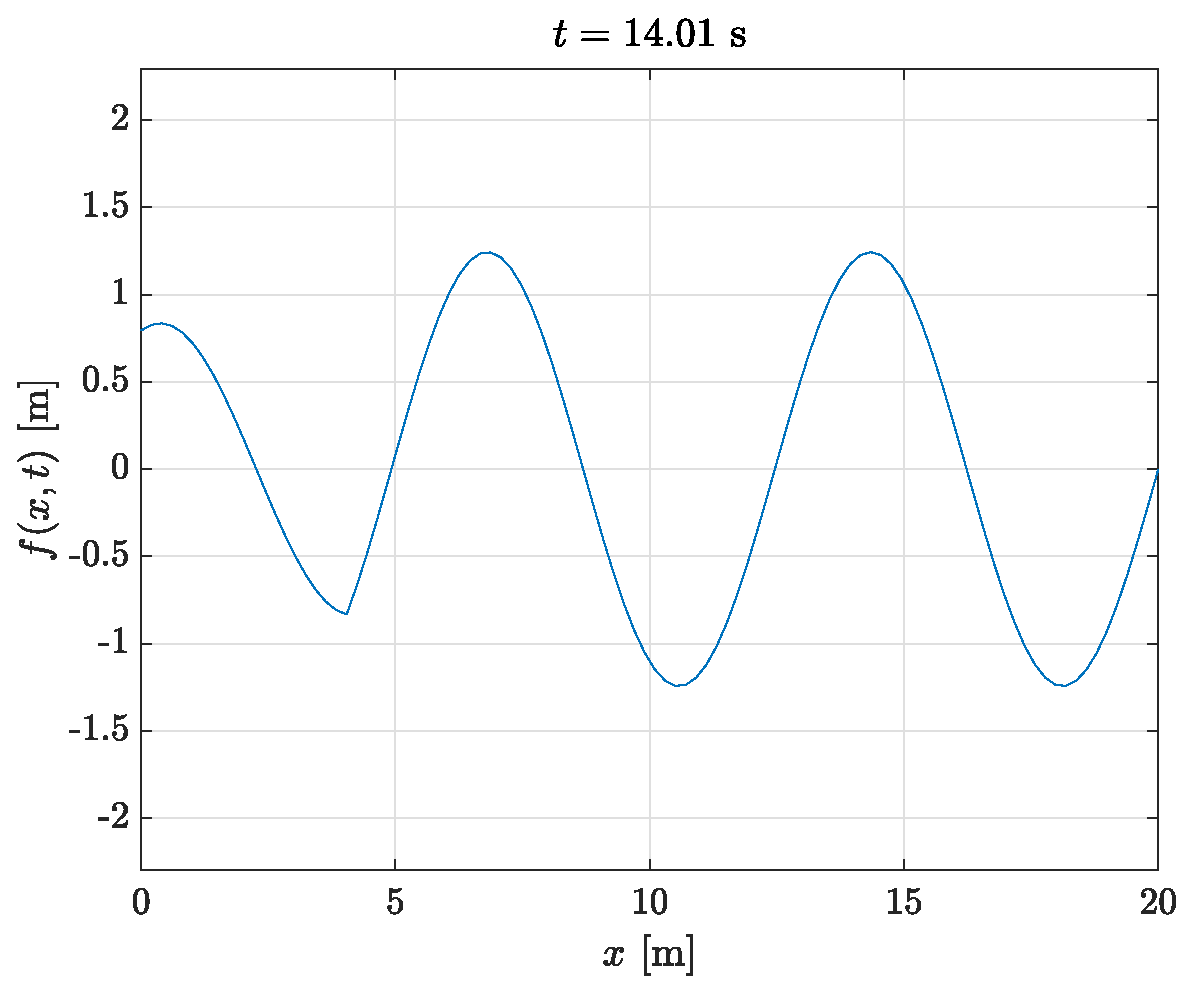
\includegraphics[width=\textwidth]{graphs/ex1ffixe.eps}
    \end{subfigure}
    ~
    \begin{subfigure}{0.55\textwidth}
    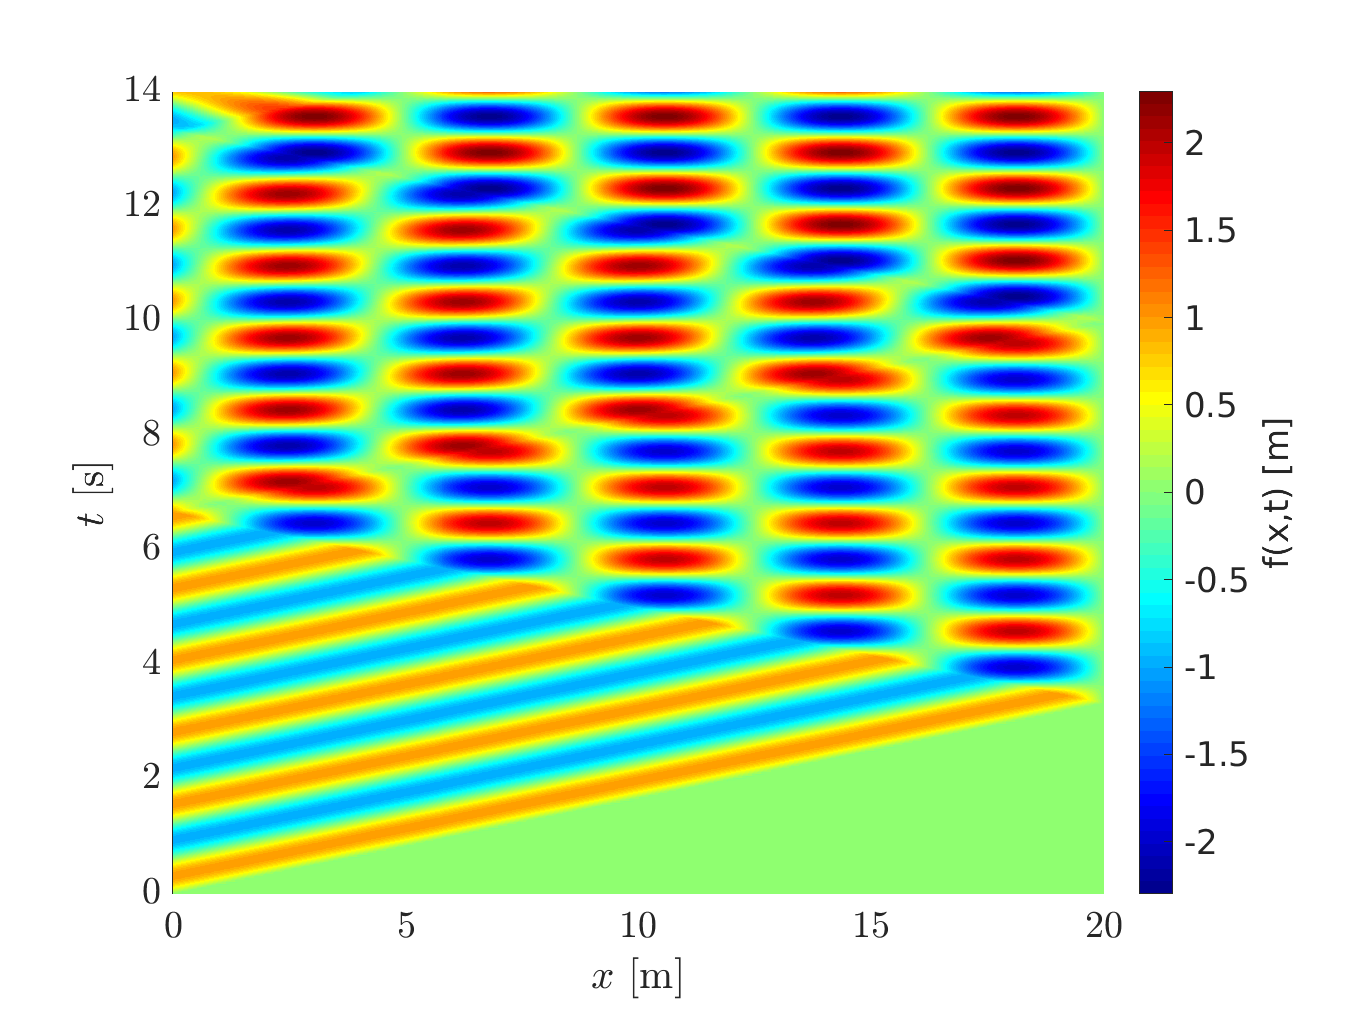
\includegraphics[width=\textwidth]{graphs/ex1xtfixe.eps}
    \end{subfigure}\

    \centering
    \begin{subfigure}{0.5\textwidth}
    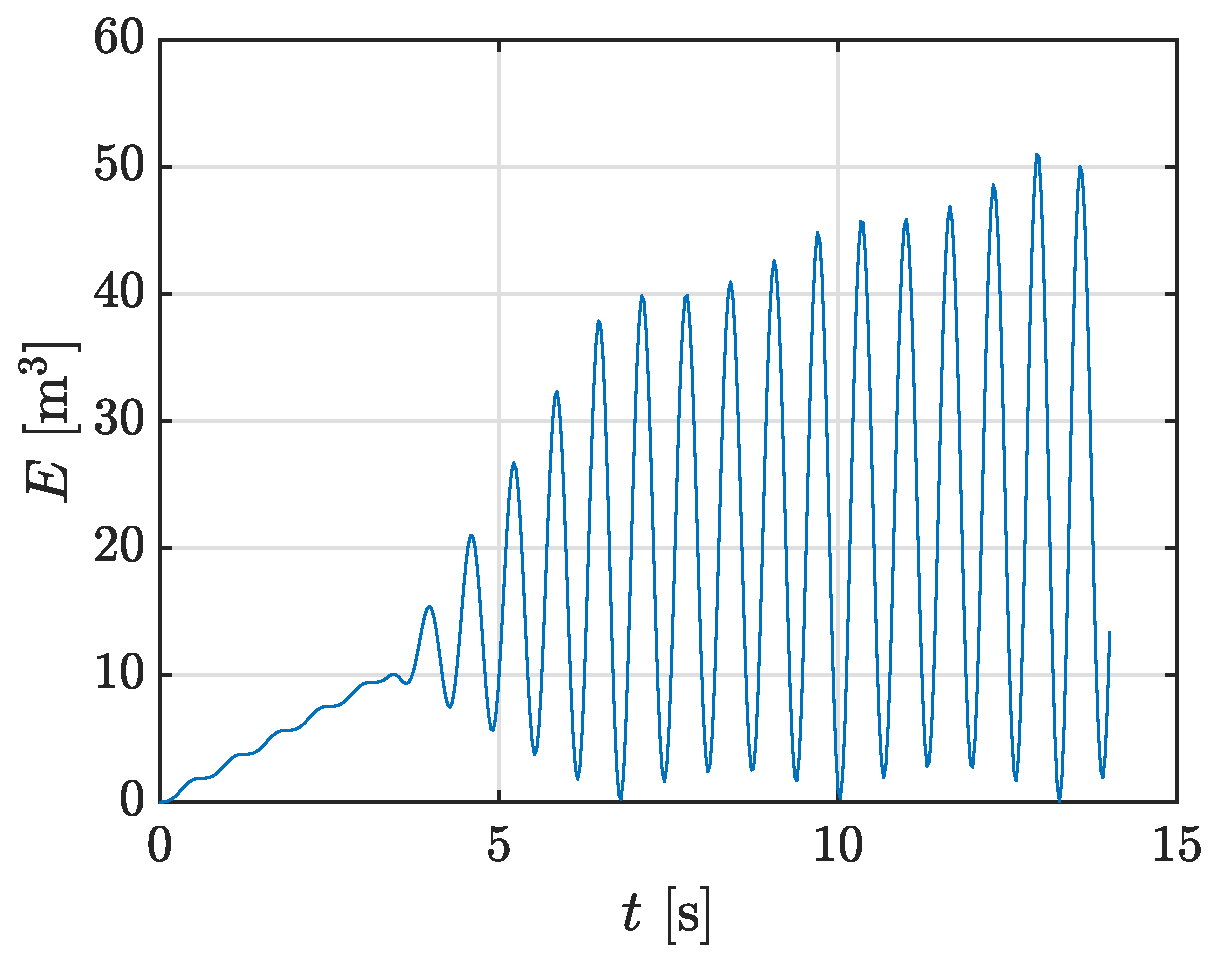
\includegraphics[width=\textwidth]{graphs/ex1Efixe.eps}
    \end{subfigure}

    \caption{Illustration of the border reflection for a the fixed right border condition}
    \label{fig:ex1fix}
    \end{figure}

    \lipsum[1-2] %TODO : Virer quand y'a le texte. C'est pour mettre de la structure.

    \begin{figure}[h!]
    \begin{subfigure}{0.5\textwidth}
    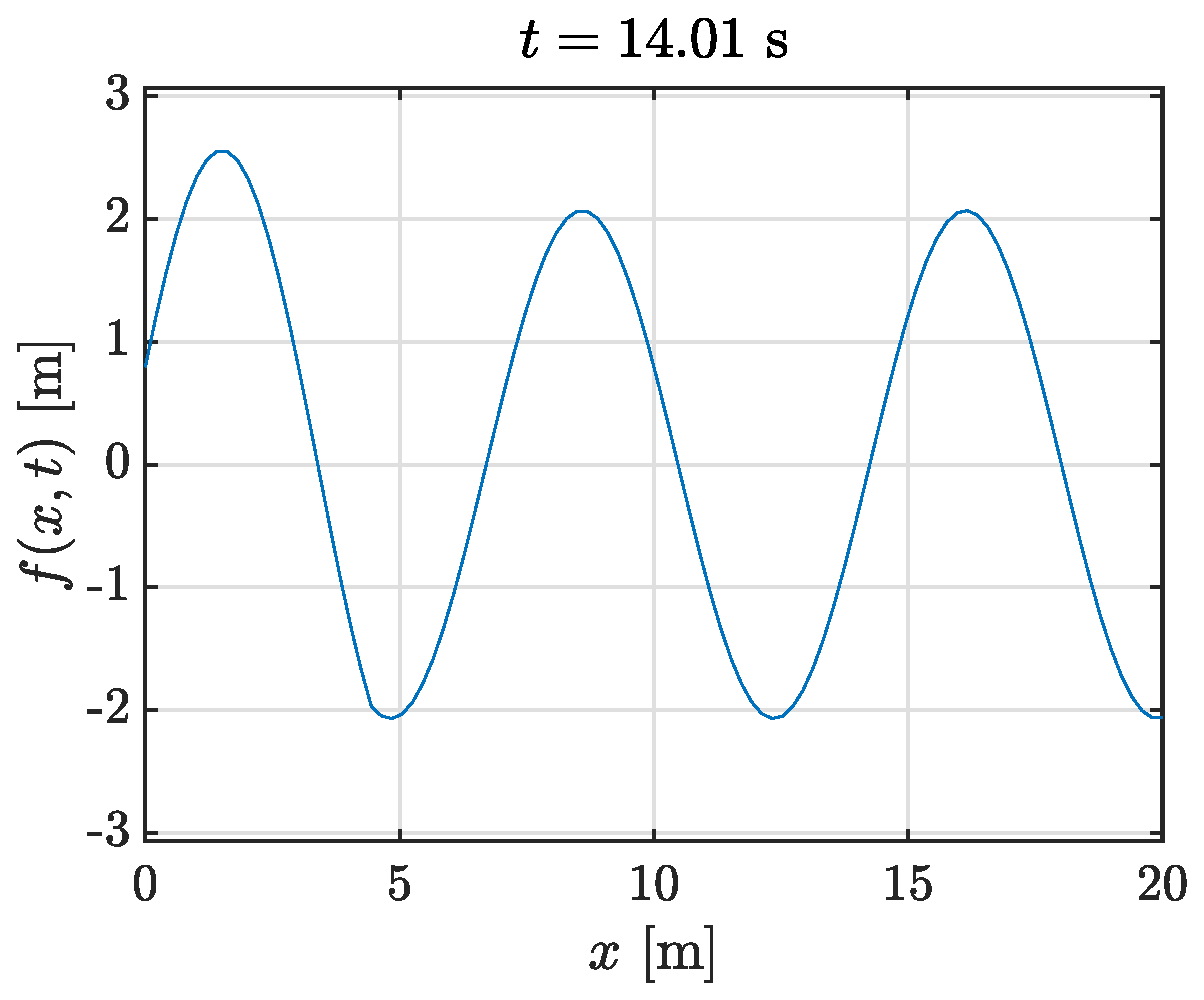
\includegraphics[width=\textwidth]{graphs/ex1flibre.eps}
    \end{subfigure}
    ~
    \begin{subfigure}{0.55\textwidth}
    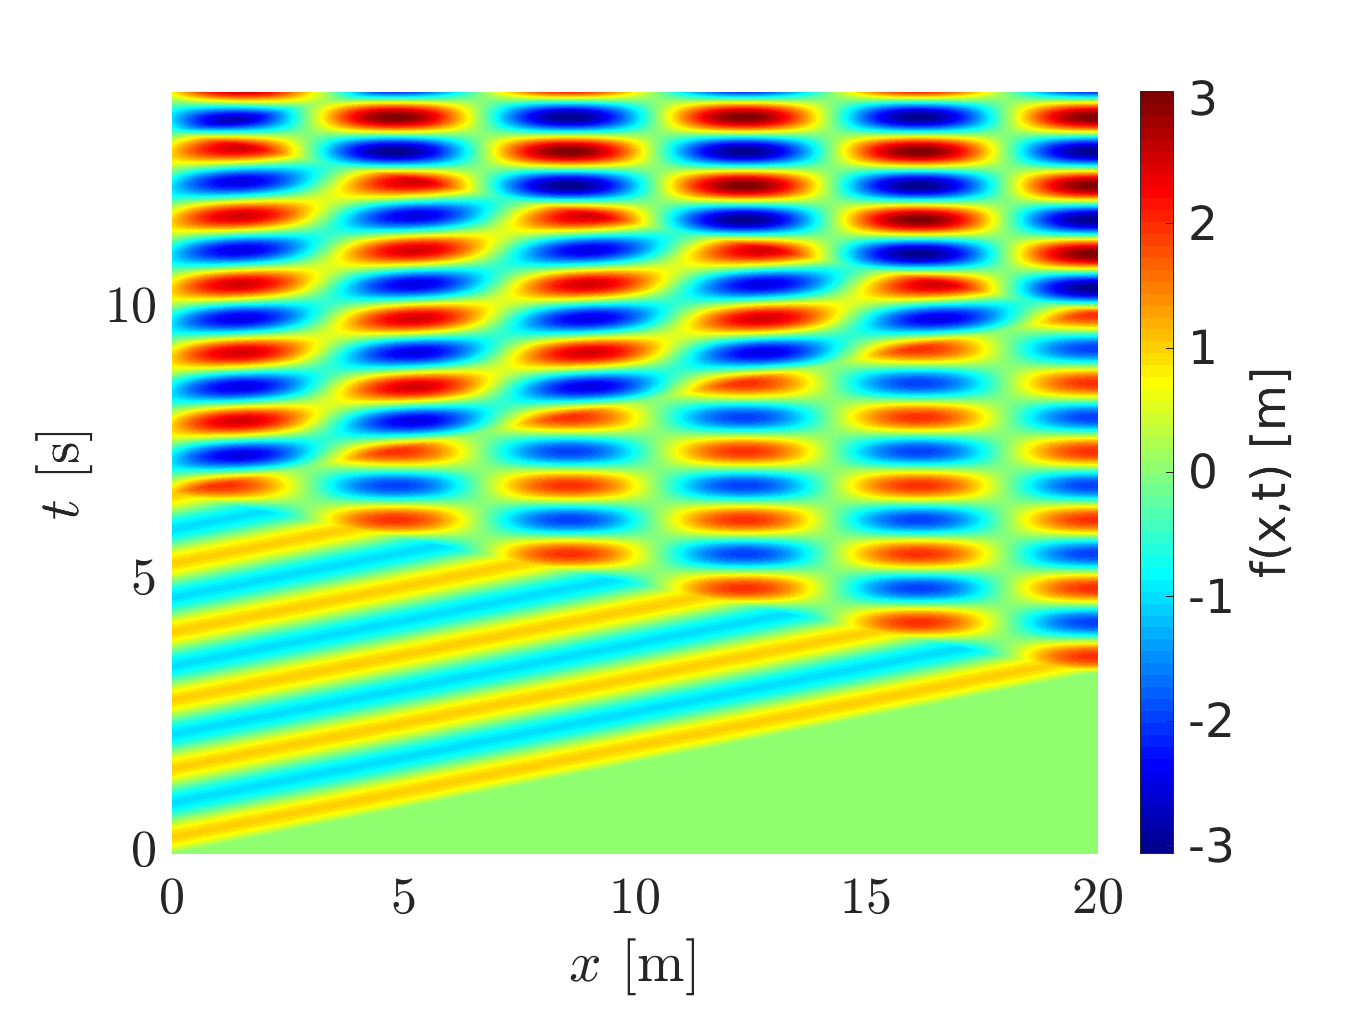
\includegraphics[width=\textwidth]{graphs/ex1xtlibre.eps}
    \end{subfigure}\

    \centering
    \begin{subfigure}{0.5\textwidth}
    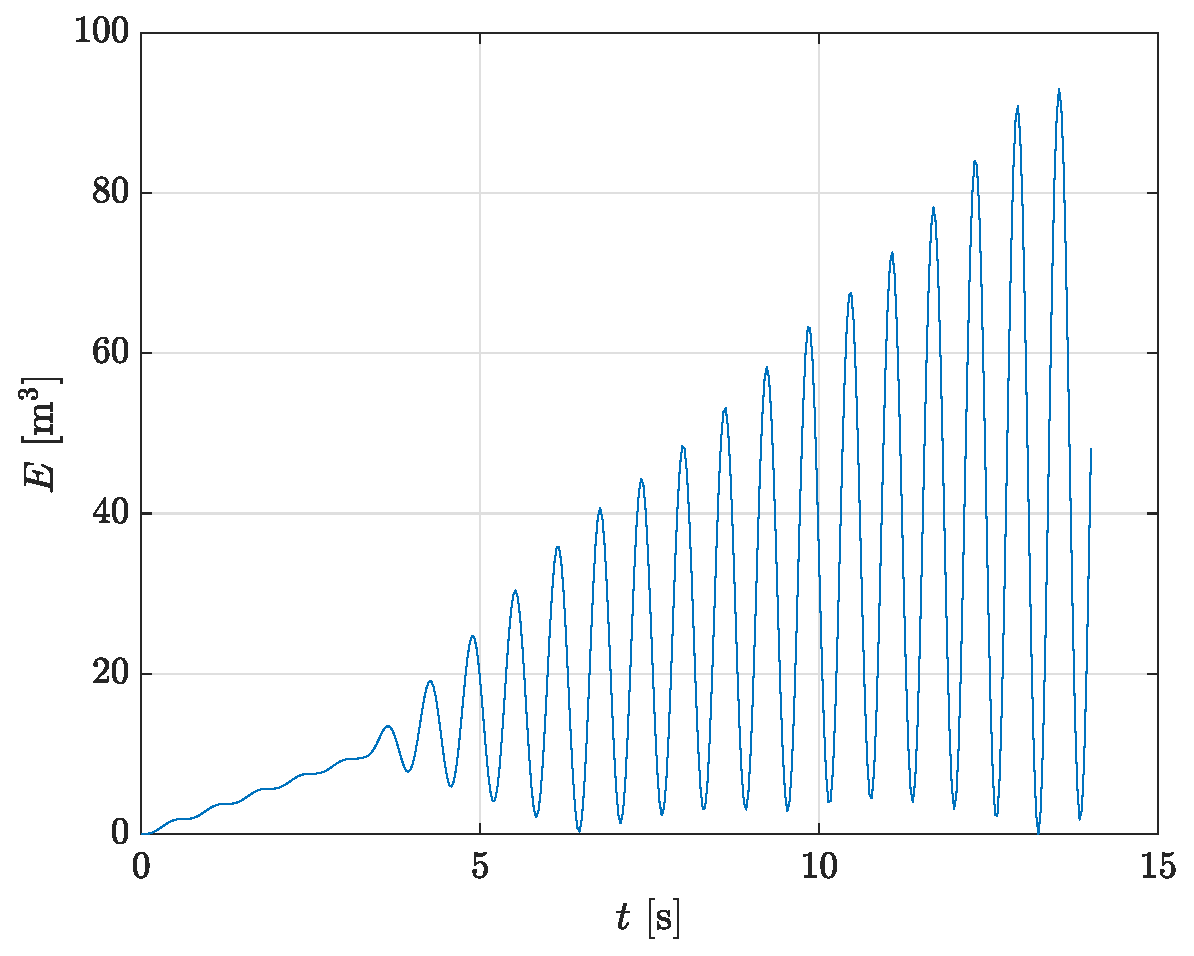
\includegraphics[width=\textwidth]{graphs/ex1Elibre.eps}
    \end{subfigure}

    \caption{Illustration of the border reflection for a the free right border condition}
    \label{fig:ex1lib}
    \end{figure}

    \lipsum[1-2] %TODO : Virer quand y'a le texte. C'est pour mettre de la structure.

    \begin{figure}[h!]
    \begin{subfigure}{0.5\textwidth}
    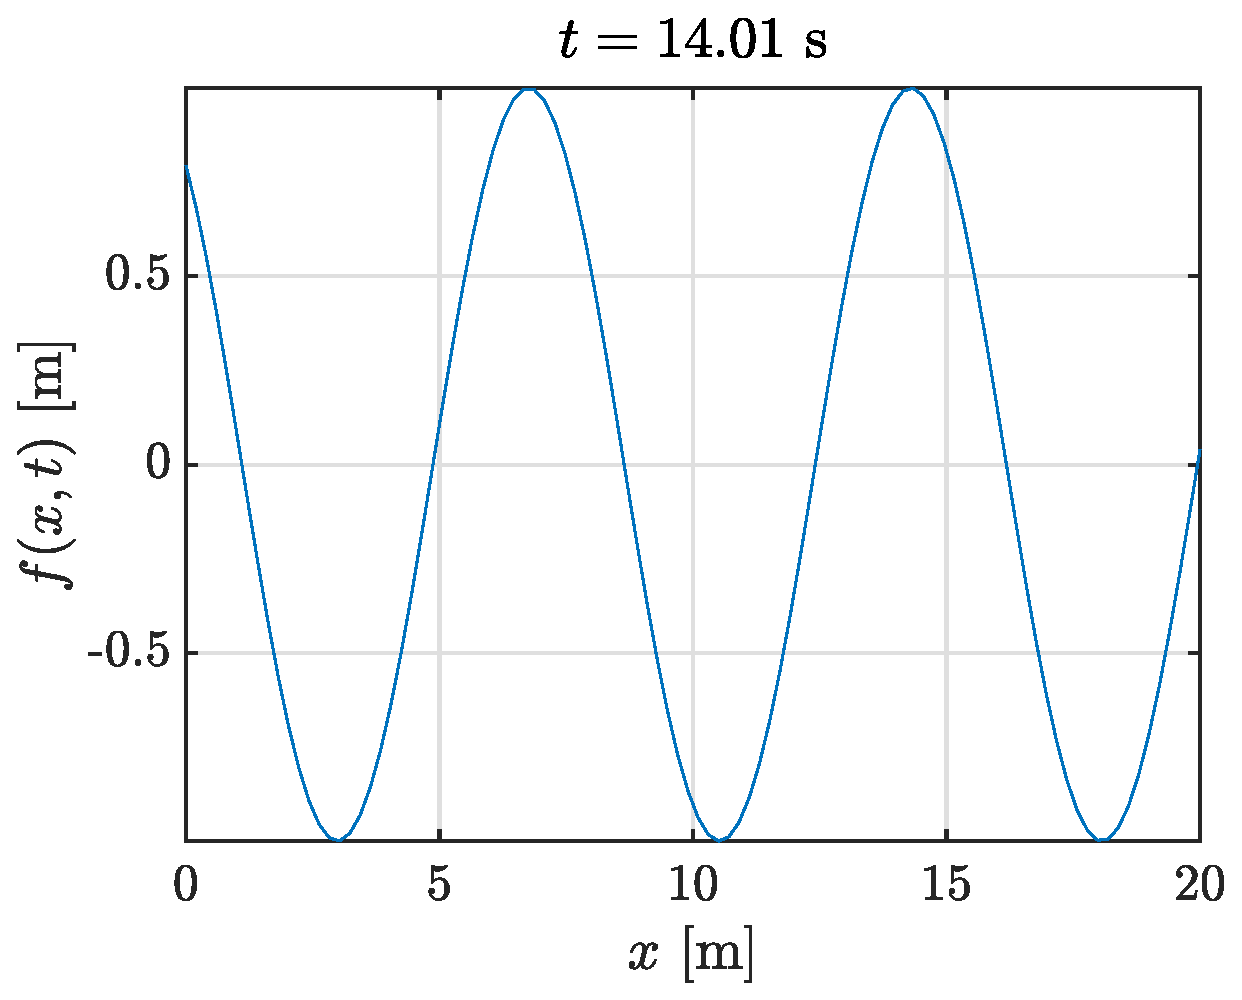
\includegraphics[width=\textwidth]{graphs/ex1fsortie.eps}
    \end{subfigure}
    ~
    \begin{subfigure}{0.55\textwidth}
    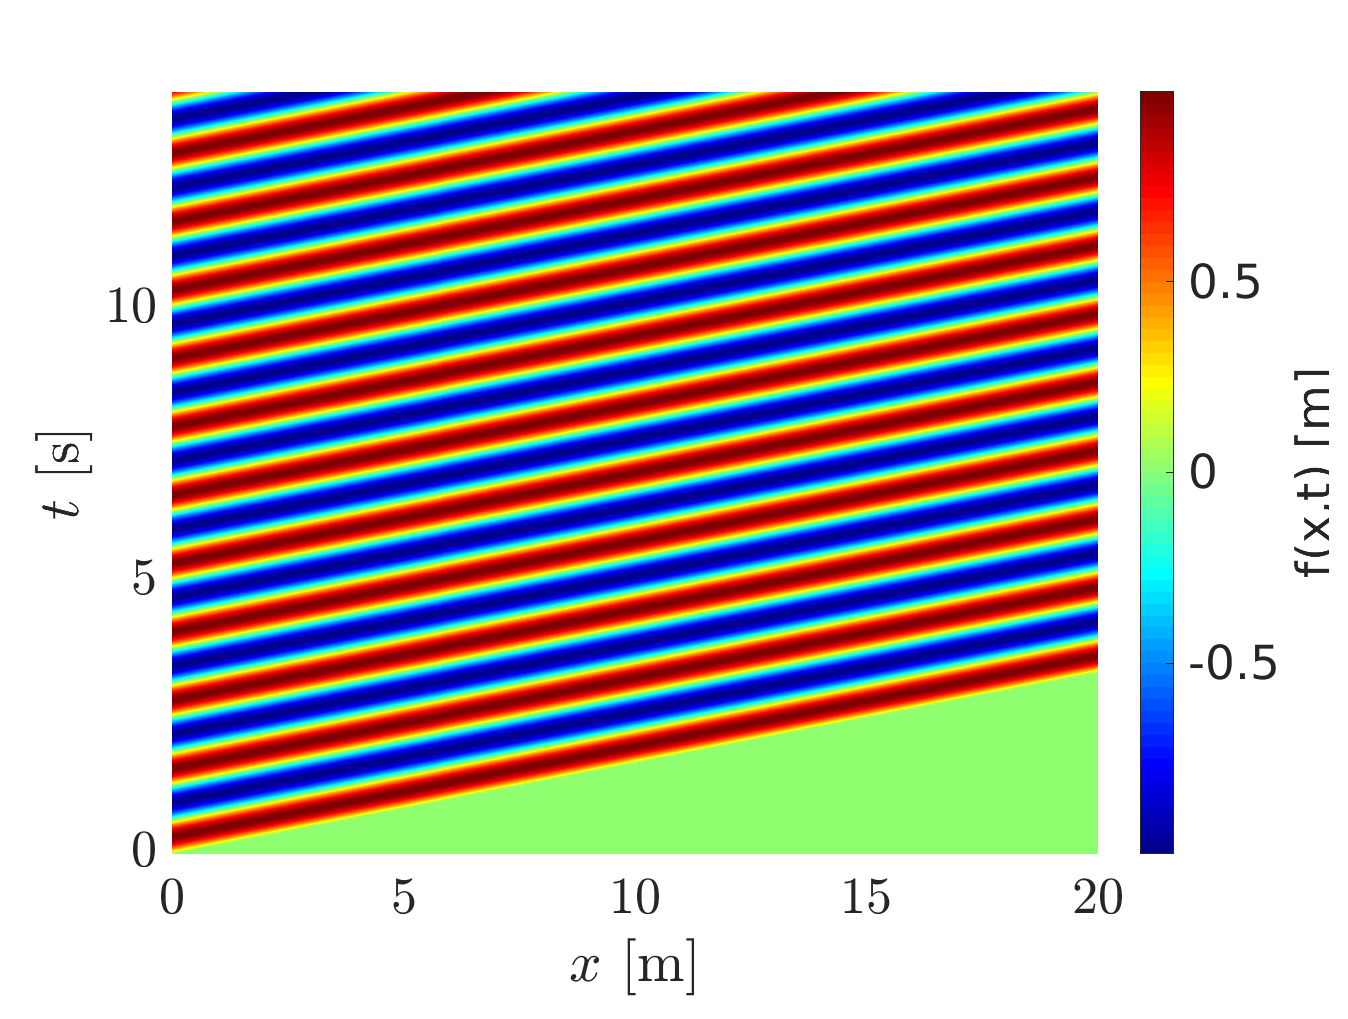
\includegraphics[width=\textwidth]{graphs/ex1xtsortie.eps}
    \end{subfigure}\

    \centering
    \begin{subfigure}{0.5\textwidth}
    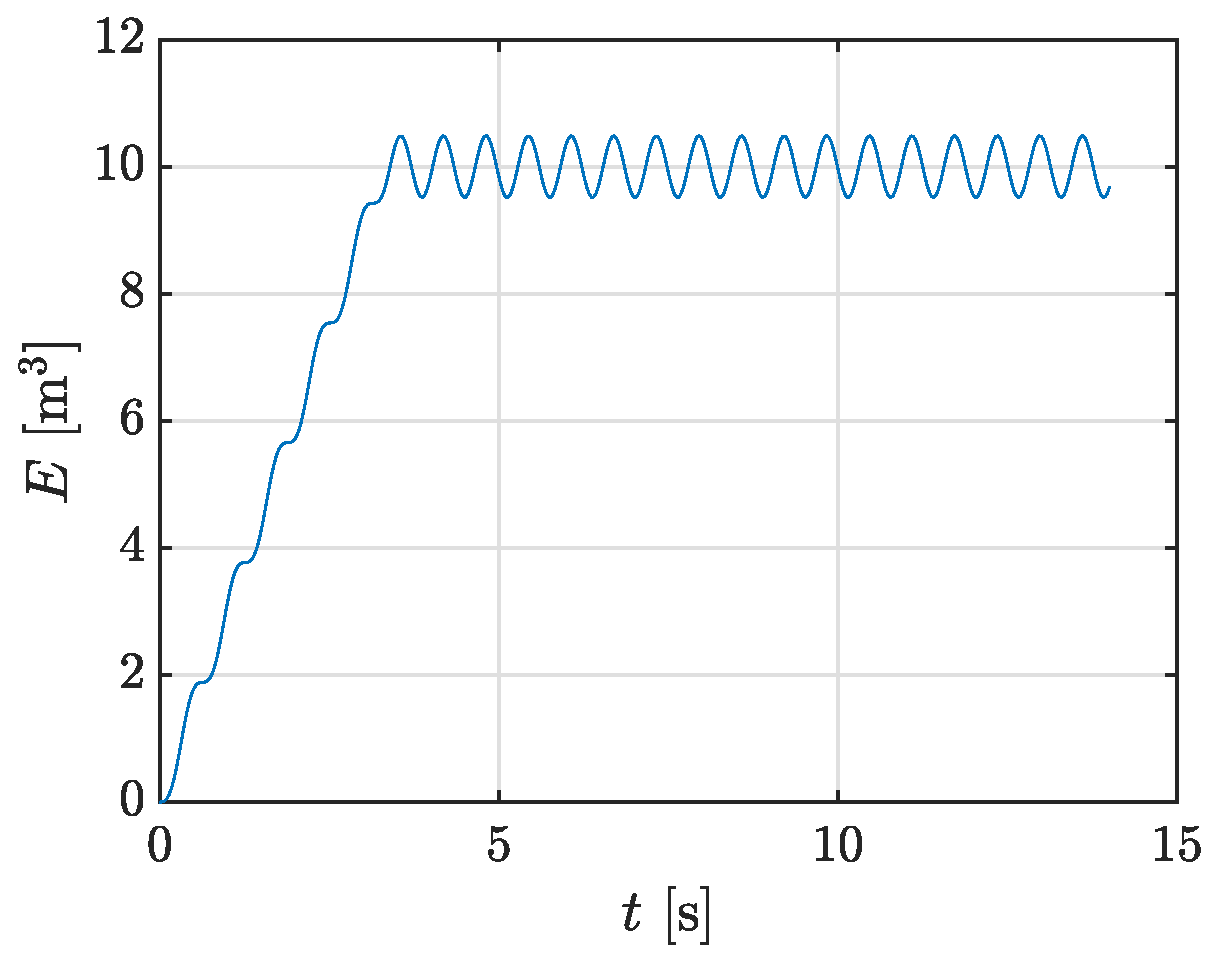
\includegraphics[width=\textwidth]{graphs/ex1Esortie.eps}
    \end{subfigure}

    \caption{Illustration of the border reflection for a the exit right border condition}
    \label{fig:ex1sor}
    \end{figure}

    \lipsum[1-2] %TODO : Virer quand y'a le texte. C'est pour mettre de la structure.

    \newpage

    \section{Tsunami}
      This section is an application of the initial problem to a tsunami.
      This time, the propagation speed is not kept constant.
      When the depth of water is low, the propagation speed of a wave can be approximated by equation \eqref{eq:prop-sp-tsunami}.

      \begin{equation}
        u\bracket{x} = \sqrt{gh\bracket{x}}
        \label{eq:prop-sp-tsunami}
      \end{equation}

      where $g=\SI{9.81}{\meter\per\square\second}$ and $h\bracket{x}$ is the depth of water, given by equation \eqref{eq:h(x)}.

      \begin{align}
        h(x)=
        \begin{cases}
          h_\text{ocean}, &x\in\sqbracket{0,x_a} \\
          h_\text{ocean} + \bracket{h_\text{reef} - h_\text{ocean}}\sin^2\bracket{\frac{\pi\bracket{x-x_a}}{2\bracket{x_b-x_a}}}, &x\in\sqbracket{x_a,x_b} \\
          h_\text{reef}, &x\in\sqbracket{x_b,x_c} \\
          h_\text{reef} - \bracket{h_\text{reef} - h_\text{ocean}}\sin^2\bracket{\frac{\pi\bracket{x_c - x}}{2\bracket{x_c-x_d}}}, &x\in\sqbracket{x_c,x_d} \\
          h_\text{ocean}, &x\in\sqbracket{x_d, L}
        \end{cases}
        \label{eq:h(x)}
      \end{align}

      where $h_\text{ocean} = \SI{8000}{\m}$, $h_\text{reef} = \SI{20}{\meter}$, $L=\SI{800}{\kilo\meter}$, $x_a = \SI{200}{\kilo\meter}$, $x_b = \SI{370}{\kilo\meter}$, $x_c=\SI{430}{\kilo\meter}$ and $x_d=\SI{600}{\kilo\meter}$.\\

      These conditions leads to figure \ref{fig:tsunami-depth}, which represents the depth $h$ of water with respect to the distance $x$.

      \begin{figure}[h]
        \centering
        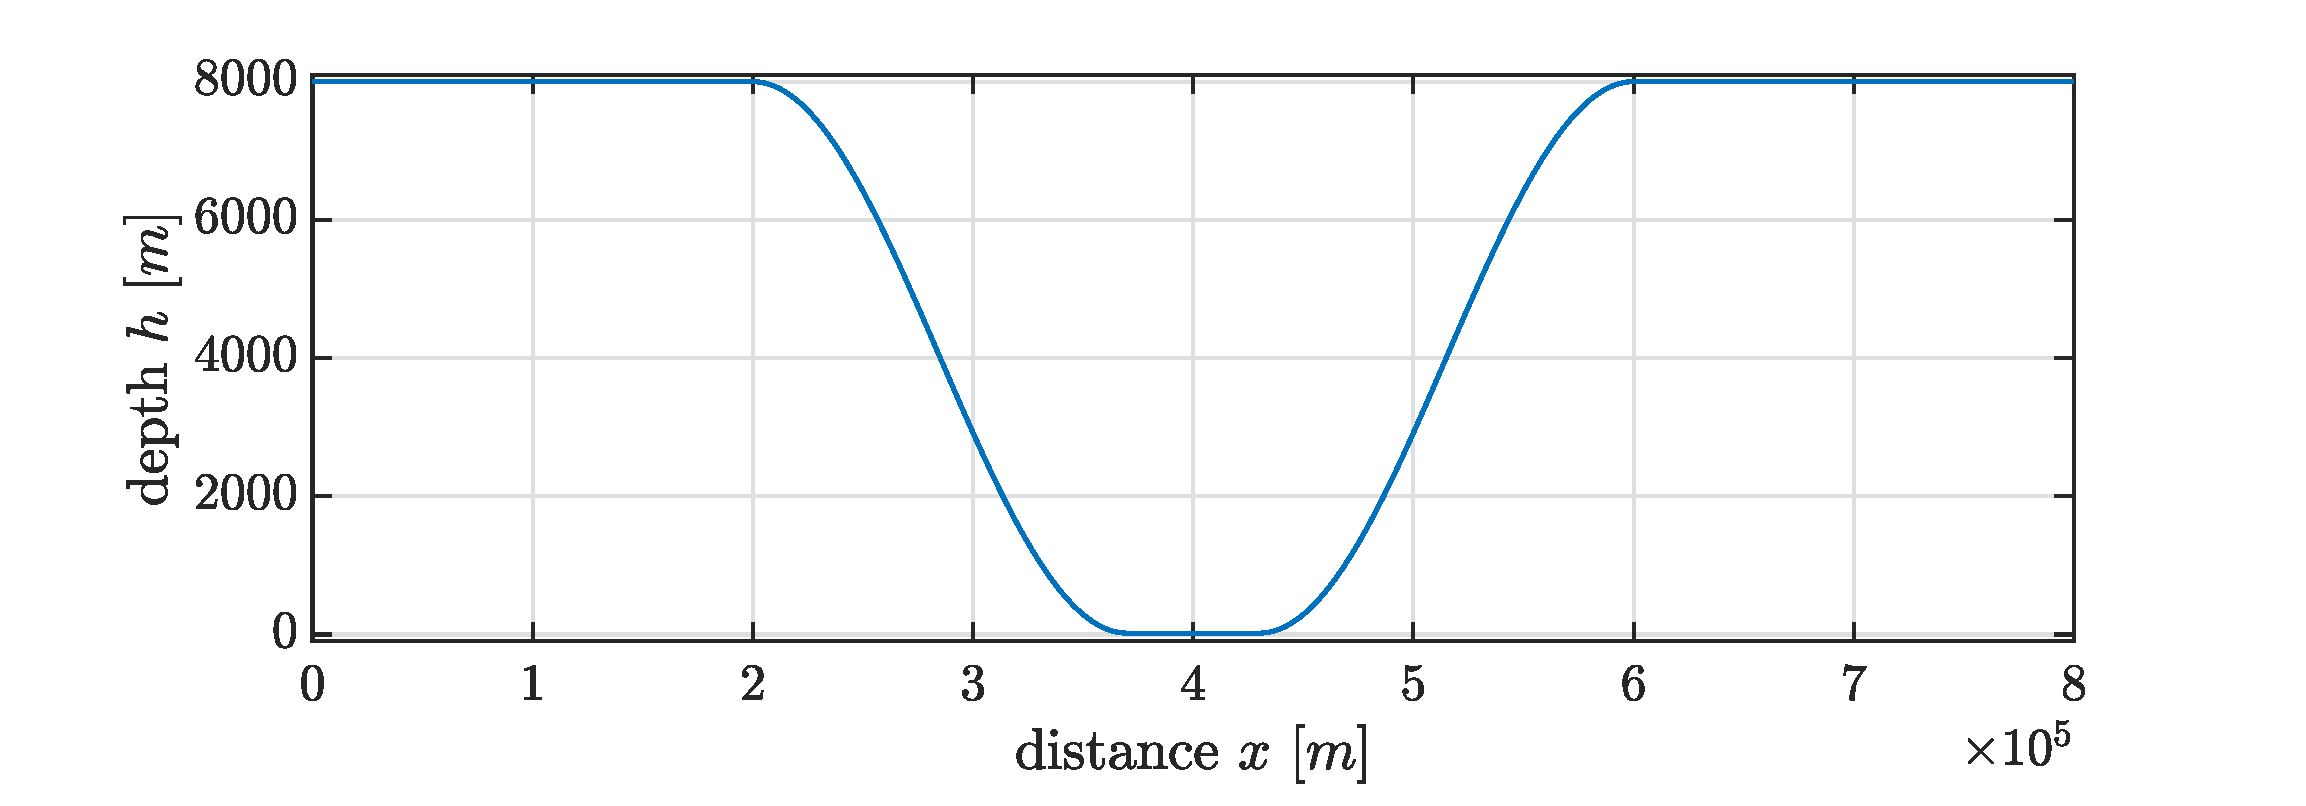
\includegraphics[width=\textwidth]{graphs/tsunami_depth.eps}
        \caption{Depth of water with respect to distance}
        \label{fig:tsunami-depth}
      \end{figure}

      The simulation will consider a single sine wave of initial amplitude \SI{1}{\meter} coming from the left border, which has a period of \SI{15}{\min} and escapes on the right border.\\

      Note that, on this section, the methods used to measure propagations speeds and amplitudes are not perfect and induces glitches in the resulting graphes.
      Thus, to improve their readability, the glitchy points were removed, as they were not useful for the study and not related to the problem.\\

      \subsection{Verifications} %TODO : Le titre est pourri
      First, the validity of all three equations will be studied through the analysis of the propagation speed of the wave, and then its amplitude.

      \subsubsection{Propagation speed}
        The goal is to check if the propagation speed of the wave indeed follows equation \eqref{eq:prop-sp-tsunami}.
        To achieve this, some treatment needs to be done to the signal, and the following method describes the way to identify and follow a single wave, as well as computing its propagation speed.
        \begin{enumerate}
          \item Find all the local maxima of the function $f(x)$ where $f$ is the amplitude and $x$ the distance, and only consider the first one.
          This will give the location of maximum of the first wave on the discretized system.
          \item Now, the problem is that the found maximum is only the one for the discretized system, and not the real maximum.
          The real maximum is not numerically foundable, thus, it needs to be approximated, through an interpolation.
          To do so, take the two points around the discrete maximum, and fit them with a parabola (2nd order interpolation).
          The real maximum can be approximated by the maximum of the parabola.
          Save the $x$ position of the maximum, and the current time.
          \item Finally, we need to detect the moment when the wave reaches the end of the domain.
          To do so, consider the three last points of the domain.
          Find the best line that fits these points, and consider its slope.
          When the slope is null, no movements is detected.
          When it is negative, a wave is starting its exit.
          When it is positive, a wave is more that half out of the domain.
          Thus, the measurements on the first wave need to be stopped when the slope gets positive.
          \item To compute the value of the propagation speed, simply consider a finite difference method to approximate $u=\dot{x}$.
          Thus, the speed is given by equation \eqref{eq:DFM-u}.
        \end{enumerate}

        \begin{equation}
          u=\frac{dx}{dt}\approx\frac{\Delta x}{\Delta t}=\frac{x_{i+1} - x_i}{t_{i+1} - t_i}
          \label{eq:DFM-u}
        \end{equation}

        This process lead to figure \ref{fig:tsunami_speed}, which gives a comparison between the theorical propagation speed of a wave, and the three equations considered.

        \begin{figure}[h]
          \centering
          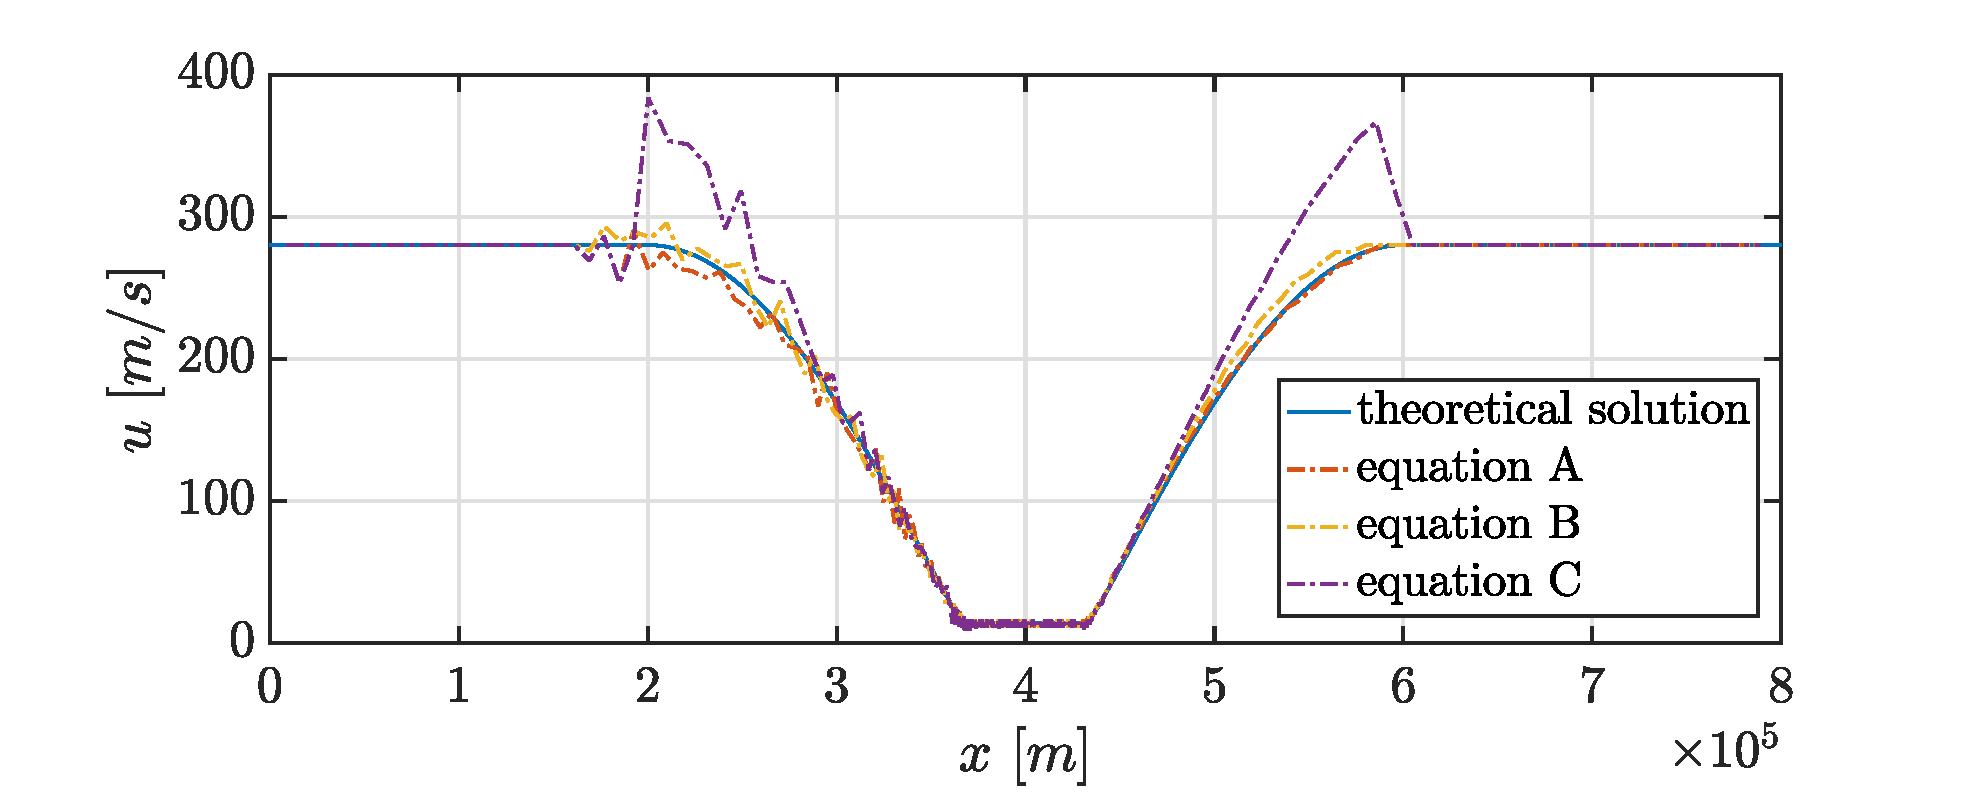
\includegraphics[width=\textwidth]{graphs/tsunami_speed.eps}
          \caption{Comparison between the theorical value of the propagation speed, and the three equations for $t_\text{fin} = \SI{10000}{\s}$ and $N_\text{points} = \num{1000}$.}
          \label{fig:tsunami_speed}
        \end{figure}

        All equations tends to follow the theorical propagation speed, but they are different from each other.
        Indeed, equation C seems to be the worst of them.
        It follows the global trend, but when the depth of water changes, the propagation speed moves further apart from the theorical value, before slowly stabilizing around it.
        Regarding equation A and B, the results are similar, as both closely follow the theorical propagation speed.
        Also, it can be observed that, before reaching the reef, all equations give an oscillation solution.
        When leaving the reef, all equation are smoother that before. %TODO : Ca vient d'où ça ? Une idée ? Faut dire un truc sinon ça sert à rien.

      \subsubsection{Amplitude}
      The analysis of the amplitude allows to check if the numerical solution indeed follows the approximation given by the WKB method.
      This method is described in depth in section \ref{sec:WKB}, and only the final solutions will be used here.

      Figure \ref{fig:tsunami-amp} gives a comparison between the amplitude of a single wave and the WKB solution for each equations.

      \begin{figure}[h]
        \centering
        \begin{subfigure}{0.45\textwidth}
          \centering
          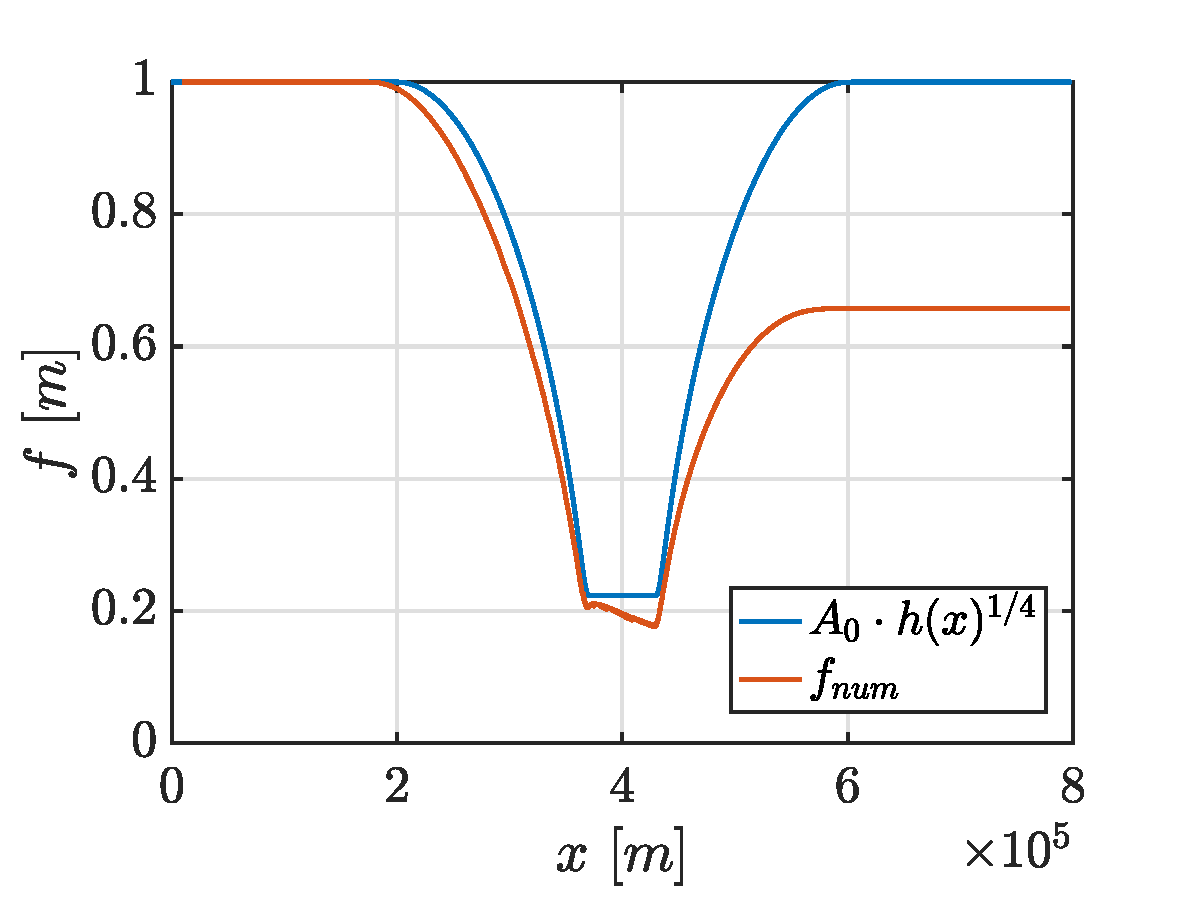
\includegraphics[width=\textwidth]{graphs/tsunami_amp_A.eps}
          \caption{Equation A using $A_0 = \num{0.0597}$}
          \label{fig:tsunami-amp-A}
        \end{subfigure}
        ~
        \begin{subfigure}{0.45\textwidth}
          \centering
          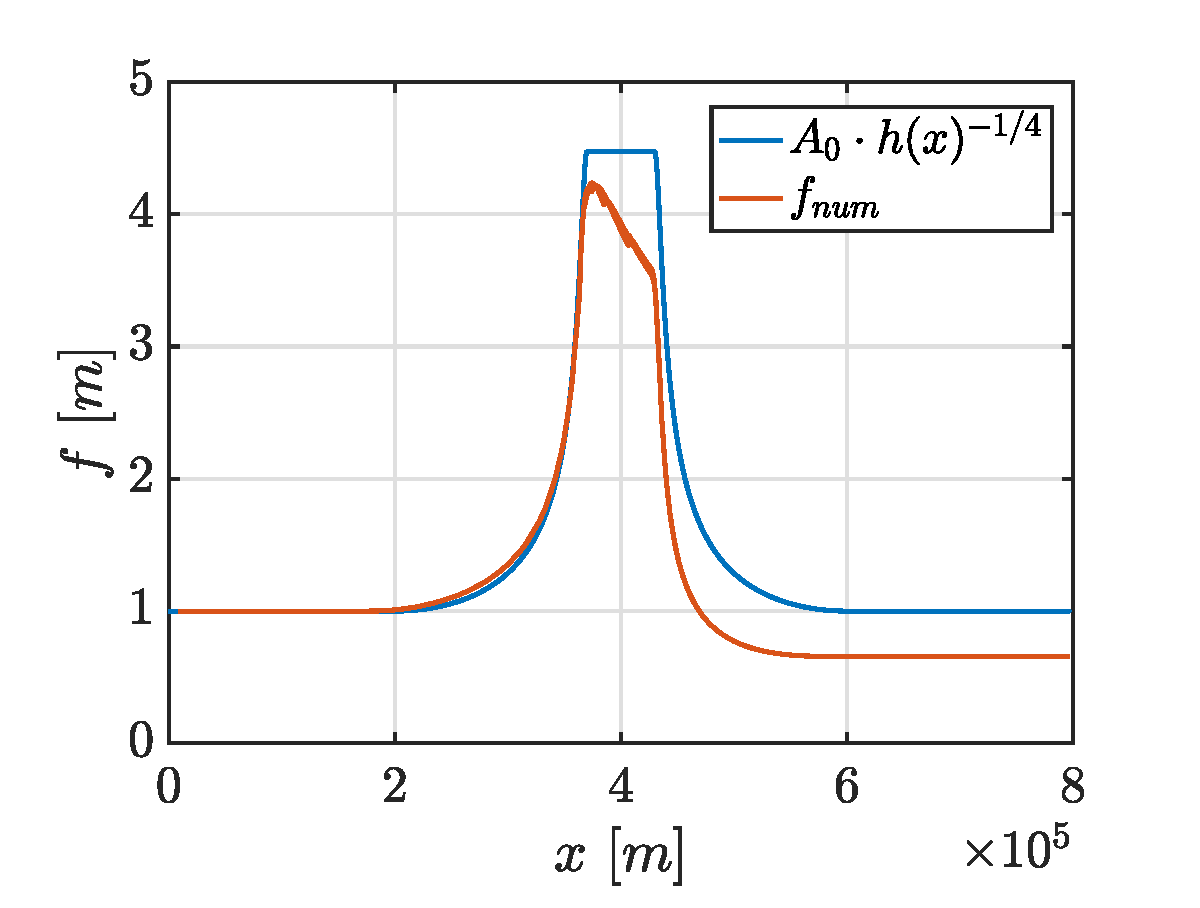
\includegraphics[width=\textwidth]{graphs/tsunami_amp_B.eps}
          \caption{Equation B using $A_0 = \num{16.7364}$}
          \label{fig:tsunami-amp-B}
        \end{subfigure}\\
        \centering
        \begin{subfigure}{0.45\textwidth}
          \centering
          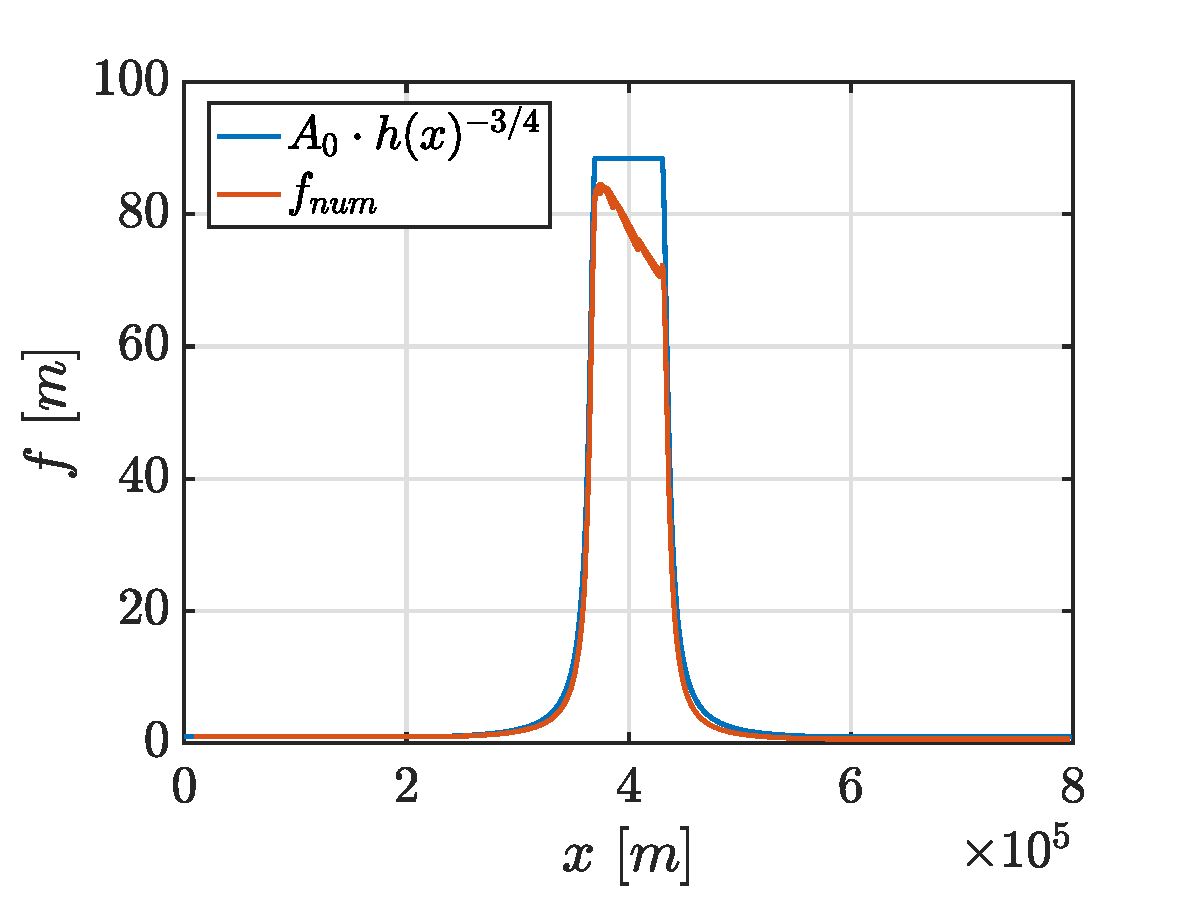
\includegraphics[width=\textwidth]{graphs/tsunami_amp_C.eps}
          \caption{Equation C using $A_0 = \num{836.8201}$}
          \label{fig:tsunami-amp-C}
        \end{subfigure}
        \caption{Verification of the WKB solution for all equations for $t_\text{fin} = \SI{10000}{\s}$ and $N_\text{points} = \num{1000}$} %TODO : C'est vrai que c'est WKB ?
        \label{fig:tsunami-amp}
      \end{figure}

      All numerical solutions follow the WKB solution for the first half.
      But after reaching the reef, all the results differ from the WKB solution in a way that can be compared to a loss of energy.
      While on the reef, the amplitude of the wave slowly reduces.
      This reduction leads to a gap between the numerical solution and the WKB solution when the wave leaves the reef.\\

      The problem may come from the WKB approximation, which makes multiple hypothesis that may not be entirely verified in the case of the tsunami.
      This method considers a general solution of the problem given by $f(x,t)=e^{-i\omega t}\hat{f}(x)$ with $\hat{f}(x) = A(x)e^{iS(x)}$.
      Two main hypothesis are therefore considered: $A(x)$ (amplitude) varies slowly, and $S(x)$ (phase) varies quickly.
      When the wave reaches the beginning of the ascent, the amplitude suddenly changes, following the curvature of the depth of the ocean.
      Thus, the variation of the amplitude is not as small as expected, which leads to the slight difference between the WKB solution and the numerical solution.
      A further analysis for the WKB solution will be done in section \ref{sec:var-xa}.

      %TODO : Dire que c'est plus le cas avec les vagues suivantes. (jojal) -> Graphe ? (il est déjà prêt)
      Aside from this problem, the analysis of the amplitude of the wave also give informations about the validity of the equations.
      Equation A (Fig. \ref{fig:tsunami-amp-A}) gives a reduction of the amplitude of a wave when approaching the reefs, which is not what happends in reality.
      If it was the case, tsunamis would not be the same problem as they are.
      On the other hand, equation C (Fig. \ref{fig:tsunami-amp-C}) gives a wave that is more that \SI{80}{\meter} high.
      As a comparison, the powerful tsunamis of 2004 in the indian ocean, cause by a magnitude 9 undersea earthquake, had waves up to \SI{30}{\meter}. \cite{wiki:tsunami-2004}
      Thus, either our wave was created by a much more energetic event, either equation C is unsuitable for this problem.\\

      In a nutshell, the verifications of all three equation by the amplitudes and the propagation speed lead to the following conclusion: equation B is the only equation that gives realistic results.


      \subsection{Varying $x_a$} \label{sec:var-xa}
      This section will study the behaviour of a single wave when parameter $x_a$ varies (see fig. \ref{fig:tsunami-depth}), in particular when it approaches $x_b$.
      All of this study is done using equation B.

      \subsubsection{Propagation speed}
        Figure \ref{fig:xa-u} gives a comparison between multiple simulations regarding the propagation speed of the wave.
        Approaching $x_a$ from $x_b$ increase the peak of speed around $x_a$.
        This problem probably comes from the multiple numerical derivative computed, using finite differences.
        At $x_a$, the curvature of the depth of ocean changes, which is not much of a problem for the cases where the slope of the depth is low.
        But when $x_a$ approaches $x_b$, the slope of the depth gets higher, which suddenly increases the variation, and causes the derivative to explode.
        This comes from the fact that the finite difference method relies on a discrete system, which here makes the gap, between one step and the next one, to explode.
        This problem can be reduced by increasing the number of points considered, which will reduce this gap at this moment, but also drastically increases the computation time of each simulation.
        %TODO : AJOUTER LA REF VERS L'ORDRE DE CONVERGENCE EN DX.

        \begin{figure}[h]
          \centering
          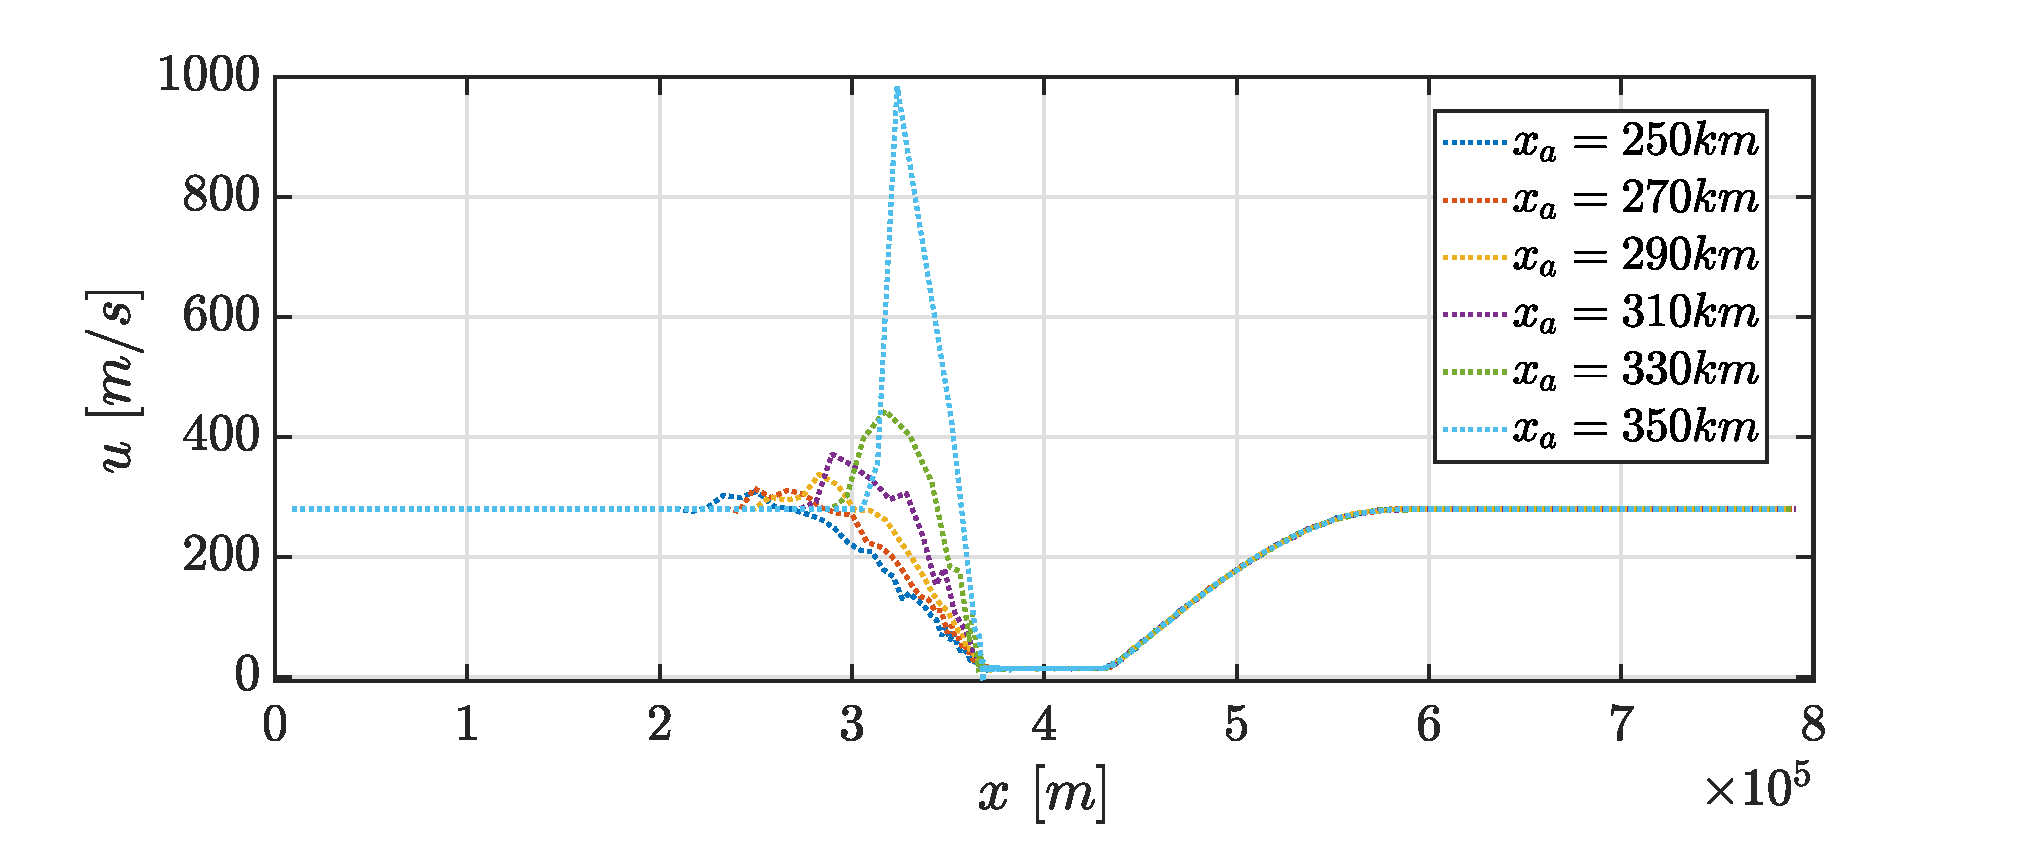
\includegraphics[width=\textwidth]{graphs/xa_u.eps}
          \caption{Comparison of propagation speeds for $t_\text{fin} = \SI{15000}{\s}$ and $N_\text{points} = \num{1000}$}
          \label{fig:xa-u}
        \end{figure}


      \subsubsection{Amplitude}
        \begin{figure}[h]
          \centering
          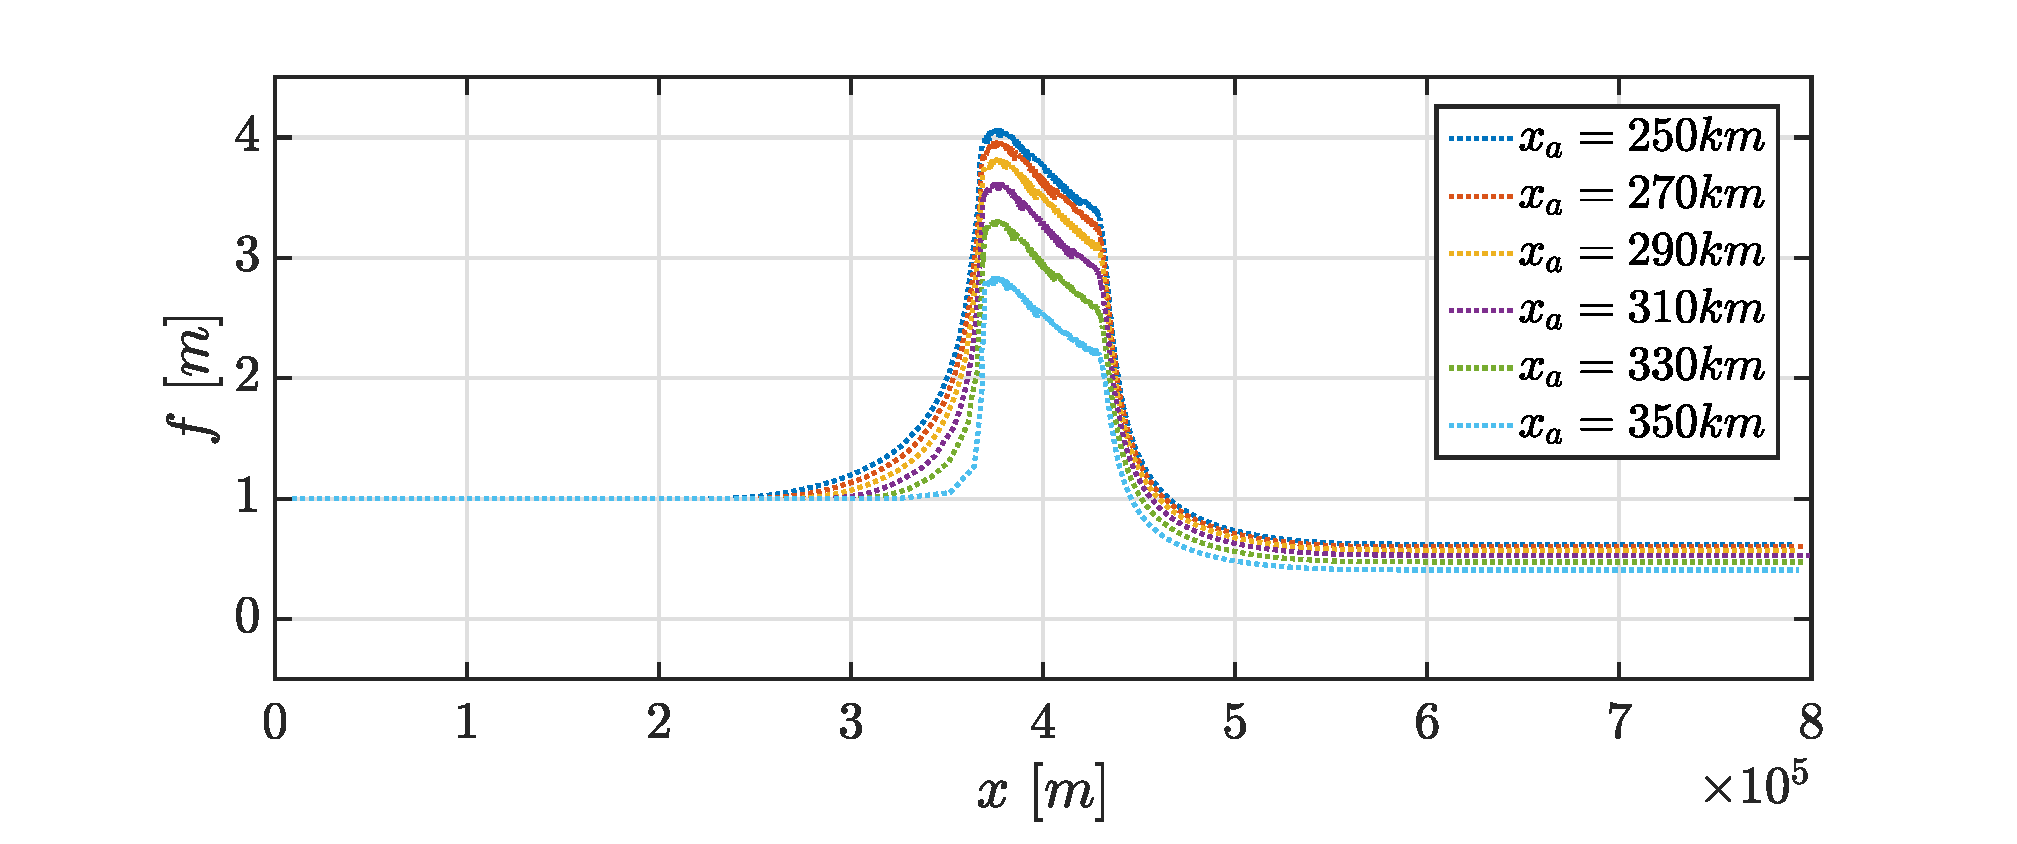
\includegraphics[width=\textwidth]{graphs/xa_f.eps}
          \caption{Comparison of amplitudes for $t_\text{fin} = \SI{15000}{\s}$ and $N_\text{points} = \num{1000}$}
          \label{fig:xa-f}
        \end{figure}

        Figure \ref{fig:xa-f} gives a comparison between multiple simulations regarding the amplitude of the wave.
        The main information here is the decrease of the maximum amplitude when $x_a$ gets closer to $x_b$.
        This result suggests that a steeper reef decreases the amplitude of a tsunami.
        This does not seem to be caused by a numerical error, as experiments showed that the difference is small between $N_\text{points}=\num{1000}$ and $N_\text{points}=\num{10000}$. %TODO : On est d'accord que y'a pas besoin de mettre le graphe ? (il est prêt, mais il montre juste que y'a peu de différences...)
        %TODO : Du coup, ça vient d'où ? Que dire de plus ?

        Figure \ref{fig:xa-WKB} gives two of the previous simulations with their WKB approximation.
        The main point here is to show that the WKB approximation is only valid for small variation of amplitude.
        Figure \ref{fig:xa-WKB-250km} shows that the numerical and the WKB solutions are not so far from each other, but figure \ref{fig:xa-WKB-350km} shows that the WKB solution is not a good approximation anymore, as its maximum is almost two times bigger than the numerical solution.
        Figure \ref{fig:xa-WKB-100m} shows that, by moving $x_a$ away from $x_b$, which reduces the variation of the amplitude, the WKB solution get really close to the numerical solution.
        Thus, this shows that the WKB solution is only valid for low-varying amplitudes.

        \begin{figure}[h]
          \centering
            \begin{subfigure}[t]{0.45\textwidth}
              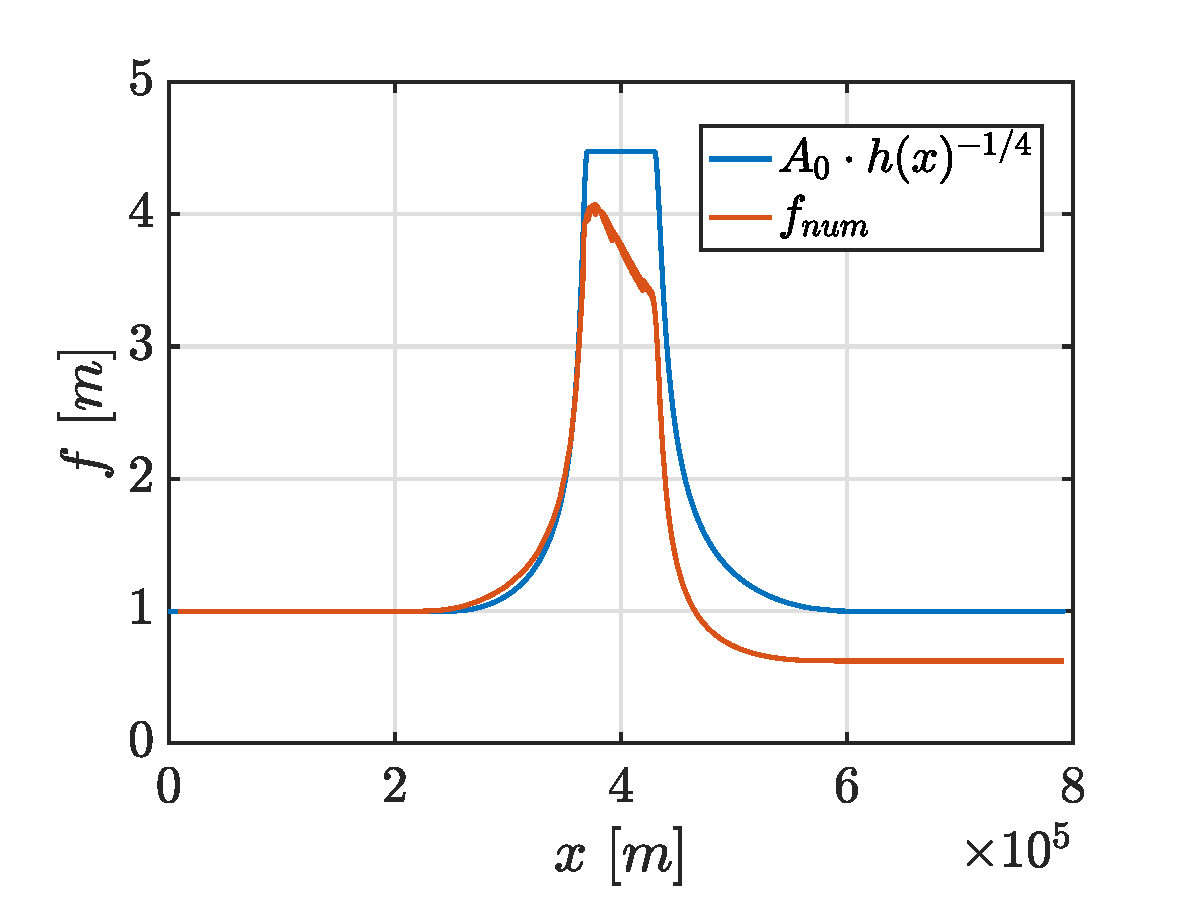
\includegraphics[width=\textwidth]{graphs/xa250000_tfin15000_f.eps}
              \caption{$x_a = \SI{250}{\kilo\meter}$}
              \label{fig:xa-WKB-250km}
            \end{subfigure}
            ~
            \begin{subfigure}[t]{0.45\textwidth}
                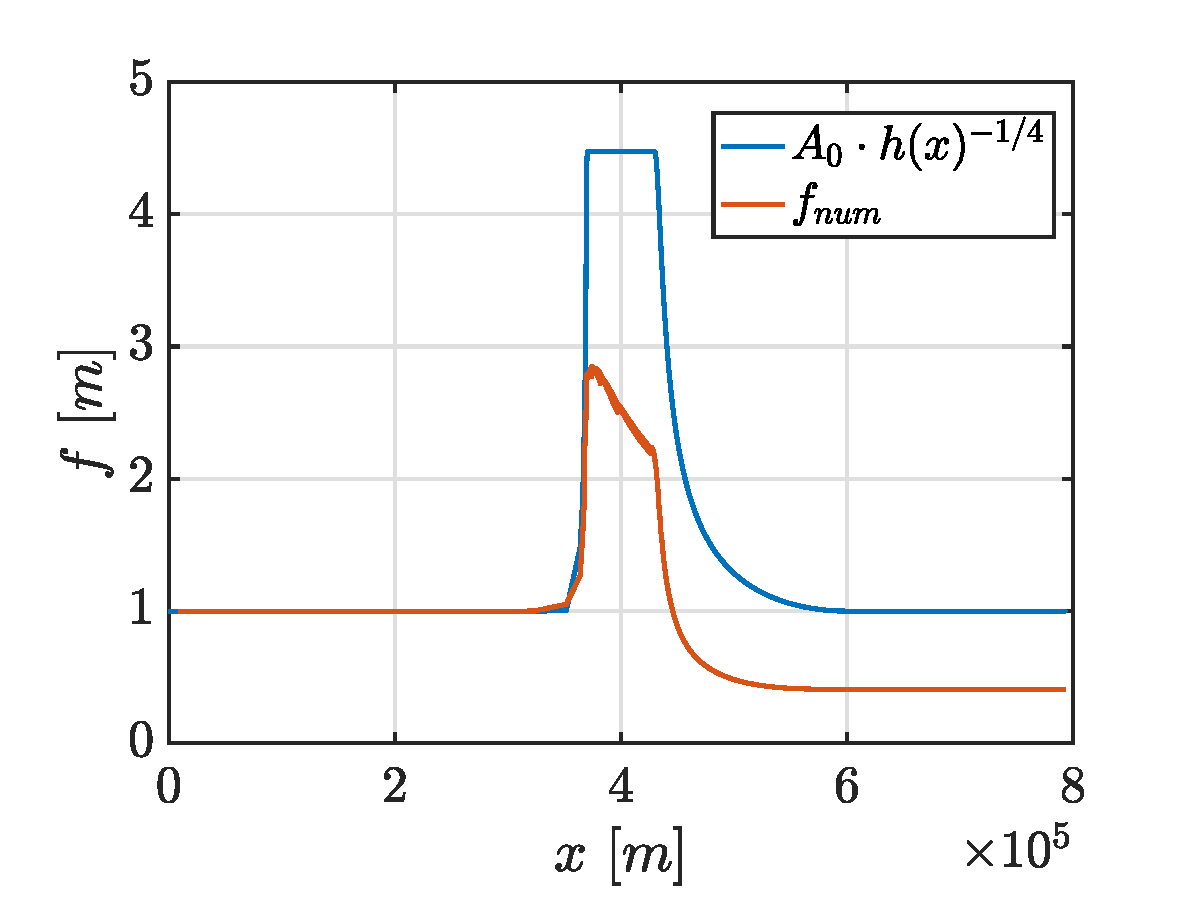
\includegraphics[width=\textwidth]{graphs/xa350000_tfin15000_f.eps}
                \caption{$x_a = \SI{350}{\kilo\meter}$}
                \label{fig:xa-WKB-350km}
            \end{subfigure}
            \\ \centering
            \begin{subfigure}[t]{0.45\textwidth}
              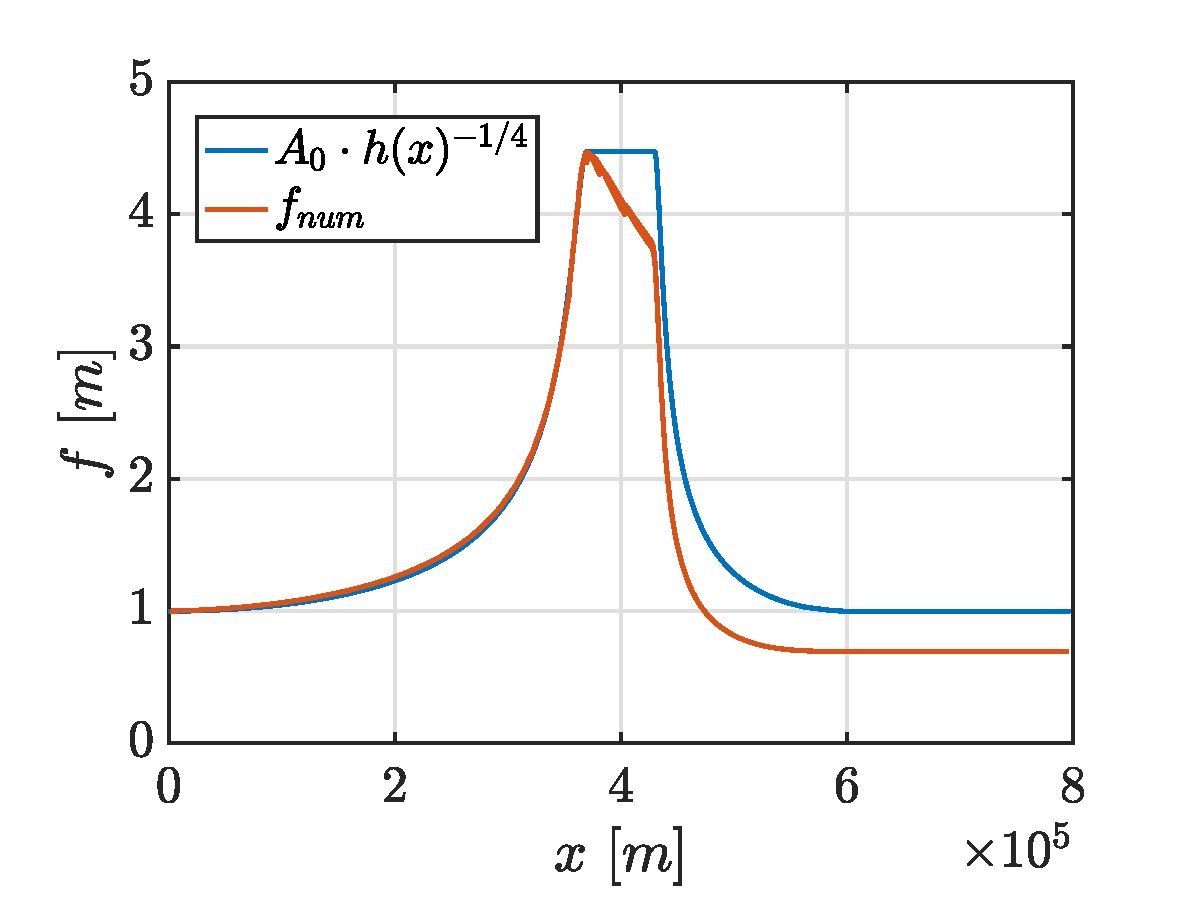
\includegraphics[width=\textwidth]{graphs/xa100_tfin15000_f.eps}
              \caption{$x_a = \SI{100}{\meter}$}
              \label{fig:xa-WKB-100m}
            \end{subfigure}

          \caption{Comparison between the WKB analysis ($A_0 \approx \num{16.74}$) and the numerical result for equation B using different $x_a$, for $t_\text{fin} = \SI{15000}{\s}$ and $N_\text{points} = 1000$}
          \label{fig:xa-WKB}
        \end{figure}

\newpage

\section{optional}
  \subsection{WKB analysis}\label{sec:WKB}
    This section give the WKB analysis for each equations.

    \subsubsection{Equation A}
      \lipsum[1-2] %TODO : Mettre le développement du WKB pour A.


    \subsubsection{Equation B}
      \begin{align*}
        \intertext{Let f(x,t) be defined by $f(x,t) = \hat{x}e^{-i\omega t}$.}
        \intertext{Using equation B and the definition of $f$:}
        \frac{\partial^2 f}{\partial t^2} &= \frac{\partial}{\partial x}\bracket{u^2\frac{\partial f}{\partial x}} \\
        -\omega^2\hat{f}\cancel{e^{-i\omega t}} &= \frac{\partial}{\partial x}\sqbracket{u^2\frac{\partial}{\partial x}\bracket{\hat{f}\cancel{e^{-i\omega t}}}}\\
        \Rightarrow -\omega^2\hat{f} &= \frac{\partial}{\partial x}\sqbracket{u^2\frac{\partial}{\partial x}\hat{f}}
        \intertext{Let $\hat{f}(x) = A(x)e^{iS(x)}$ be an ansatz, where $A(x)$ slowly varies, and $S(x)$ quickly varies. Thus:}
        -\omega^2 Ae^{iS} = \frac{\partial}{\partial x}\sqbracket{u^2\frac{\partial}{\partial x}\bracket{Ae^{iS}}} &= \frac{\partial}{\partial x}\sqbracket{u^2\bracket{A'e^{iS} + AiS'e^{iS}}}\\
        = \underbrace{2uu'}_{\bracket{u^2}'}\sqbracket{A'e^{iS} + Ais'e^{iS}} &+ u^2\sqbracket{A''e^{iS} + A'S'ie^{iS} + A'S'ie^{iS} + AS''ie^{iS} + AS'^2e^{iS}}\\
        \intertext{Now, the elements need to be grouped by "variation order". This variation order $n$ is defined by $\epsilon^n$, and $n$ increases by $1$ each time a derivation occures. Also, note that $\epsilon$ works the same as any real number, which means $\epsilon^n\cdot\epsilon^m = \epsilon^{nm}$. Thus, by hypothesis, let $A(x)\sim\epsilon^0$ and $S'(x)\sim\epsilon^1$. This leads to:}
        \underbrace{-\omega^2A}_{\epsilon^0} = \underbrace{-(S')^2u^2A}_{\epsilon^0} &+ \underbrace{i\bracket{2u^2A'S'+u^2AS''+(u^2)'AS'}}_{\epsilon^1} + \underbrace{u^2A''+(u^2)'A'}_{\epsilon^2}\\
        \intertext{By  equalizing the variation order, three equations are obtained.}
        \intertext{From $\epsilon^0$ and by defining $k(x) = \frac{dS}{dx}$, which is the local wave number:}
        \cancel{-}\omega^2\cancel{A} &= \cancel{-}(S')^2u^2\cancel{A} \Rightarrow \boxed{S'(x)=k(x)=\frac{\omega}{u(x)}}\\
        \intertext{From $\epsilon^1$:}
        2u^2A'S'+u^2AS''+(u^2)'AS' &= 0\\
        2u^{\cancel{2}}A'\frac{\cancel{\omega}}{\cancel{u}}+u^2A\bracket{\frac{\cancel{\omega}}{u}}'+(u^2)'A\frac{\cancel{\omega}}{u} &= 0\\
        2uA' + \bracket{u^{\cancel{2}}\frac{1}{\cancel{u}}}'A &= 0 \Rightarrow \boxed{2uA' + u'A = 0}\\
        \intertext{This differential equation can be solved. Suppose $A\neq0$ and $u\neq0~\forall x$.}
        2uA' &= - u'A~\Leftrightarrow~\frac{A'}{A} = -\frac{u'}{2u}\\
        \Leftrightarrow~\bracket{\log A}' &= -\frac{1}{2}\bracket{\log u}'~\Leftrightarrow~\log A+\frac{1}{2}\log u = C\text{, where $C$ is a constant.}\\
        \intertext{Now, apply $\exp(\cdot)$ on both sides}
        A\sqrt{u} = e^C &:= A_0\\
        \intertext{This leads to the result, equation \eqref{eq:WKB-B}.}
      \end{align*}

      \begin{equation}
        \boxed{A=\frac{A_0}{\sqrt{u}}} %TODO : Ajouter une égalité en changeamt u avec son approximation.
        \label{eq:WKB-B}
      \end{equation}

    \subsubsection{Equation C}
        \lipsum[1-2] %TODO : Mettre le développement du WKB pour C.





  \newpage
  \begin{thebibliography}{99}
    \bibitem{wiki:tsunami-2004} Wikipedia contributors. (2019, April 6). 2004 Indian Ocean earthquake and tsunami. In Wikipedia, The Free Encyclopedia. Retrieved 18:57, April 7, 2019, from \url{https://en.wikipedia.org/w/index.php?title=2004_Indian_Ocean_earthquake_and_tsunami&oldid=891255016}


  \end{thebibliography}

\end{document}
